\documentclass[a4paper]{article}

\usepackage[text={16cm, 25cm}, left=2.8cm, top=1.8cm]{geometry}
\usepackage[T1]{fontenc}
\usepackage[utf8x]{inputenc}
\usepackage[linguistics]{forest}
\usepackage[hidelinks,unicode]{hyperref}
\usepackage[czech]{babel}
\usepackage{color}
\usepackage{parskip}

\usepackage{tikz}
\def\checkmark{\tikz\fill[green,scale=0.4](0,.35) -- (.25,0) -- (1,.7) -- (.25,.15) -- cycle;} 

\usepackage{multicol}

\usepackage{amsmath}
\usepackage{amsthm}

\theoremstyle{definition}
\newtheorem{definition}{Definice}

\newcounter{rulenum}
\setcounter{rulenum}{1}
\newcommand{\nter}[1]{\textcolor{blue}{\,#1\,}}
\newcommand{\ter}[1]{\textbf{\textcolor{red}{\,#1\,}}}
\newcommand{\grule}[2]{{\small\arabic{rulenum}. \stepcounter{rulenum} \nter{#1} $\to$ #2}\\}
\newcommand{\drule}[2]{\checkmark \grule{#1}{#2}}


\title{Gramatická pravidla jazyka IFJ21}

\begin{document}
	
\begin{titlepage}
	\begin{center}
	
\includegraphics[width=\linewidth]{inc/FIT_logo.pdf}\\
	\vspace{\stretch{0.2}}
	{\Huge
		Implementace překladače imperativního jazyka IFJ21\\[0.5em] Tým 005, varianta I.
	}\\
	\vspace{\stretch{0.8}}
	\begin{minipage}{0.6\linewidth}
		\begin{center}
		\Large
		\begin{tabular}{l c r}
			\textbf{Tadeáš Vintrlík} & \texttt{xvintr04} & $25\%$ \\
			Kryštof Albrecht & \texttt{xalbre05} & $25\%$ \\
			Josef Škorpík & \texttt{xskorp07} & $25\%$ \\
			Jakub Kozubek & \texttt{xkozub07} & $25\%$ \\
		\end{tabular}
		\end{center}
	\end{minipage}
	\end{center}
	\vfill
	\today
\end{titlepage}

\newpage

\tableofcontents

\newpage

\section{Rozdělení práce v týmu}

Při práci na projektu jsme využívali metodu párového programování. Komunikace probíhala přes Discord a pravidelně jsme se scházeli i osobně.

Pro verzování projektu byl využit GitHub.

\subsection{Tadeáš Vintrlík}

\begin{itemize}
	\item Tabulka symbolů

	\item Abstraktní datové typy - seznam, zásobník, AVL stromy

	\item Testy pro ADT a syntaktický analyzátor
	
	\item Generování kódu

	\item Sémantické kontroly
	
	\item Precedenční analyzátor
\end{itemize}

\subsection{Kryštof Albrecht}

\begin{itemize}
	\item Lexikální analyzátor

	\item Syntaktický analyzátor shora-dolů
	
	\item LL-gramatika
\end{itemize}

\subsection{Josef Škorpík}

\begin{itemize}
	\item Lexikální analyzátor
	
	\item Syntaktický analyzátor shora-dolů
\end{itemize}

\subsection{Jakub Kozubek}

\begin{itemize}
	\item Generování kódu
	
	\item ADT dynamický řetězec

	\item Testy pro lexikální analyzátor

	\item Precedenční tabulka
\end{itemize}

\newpage

\section{Návrh překladače}



\subsection{Lexikální analyzátor}

Lexikální analyzátor je implementován v souboru \texttt{scanner.c}.

Implementuje mimo jiné i zásobník tokenů, aby mohl syntaktický analyzátor vracet nechtěné tokeny zpět (\texttt{unget\_token(T\_token* token)}).

\subsubsection{Diagram konečného automatu}

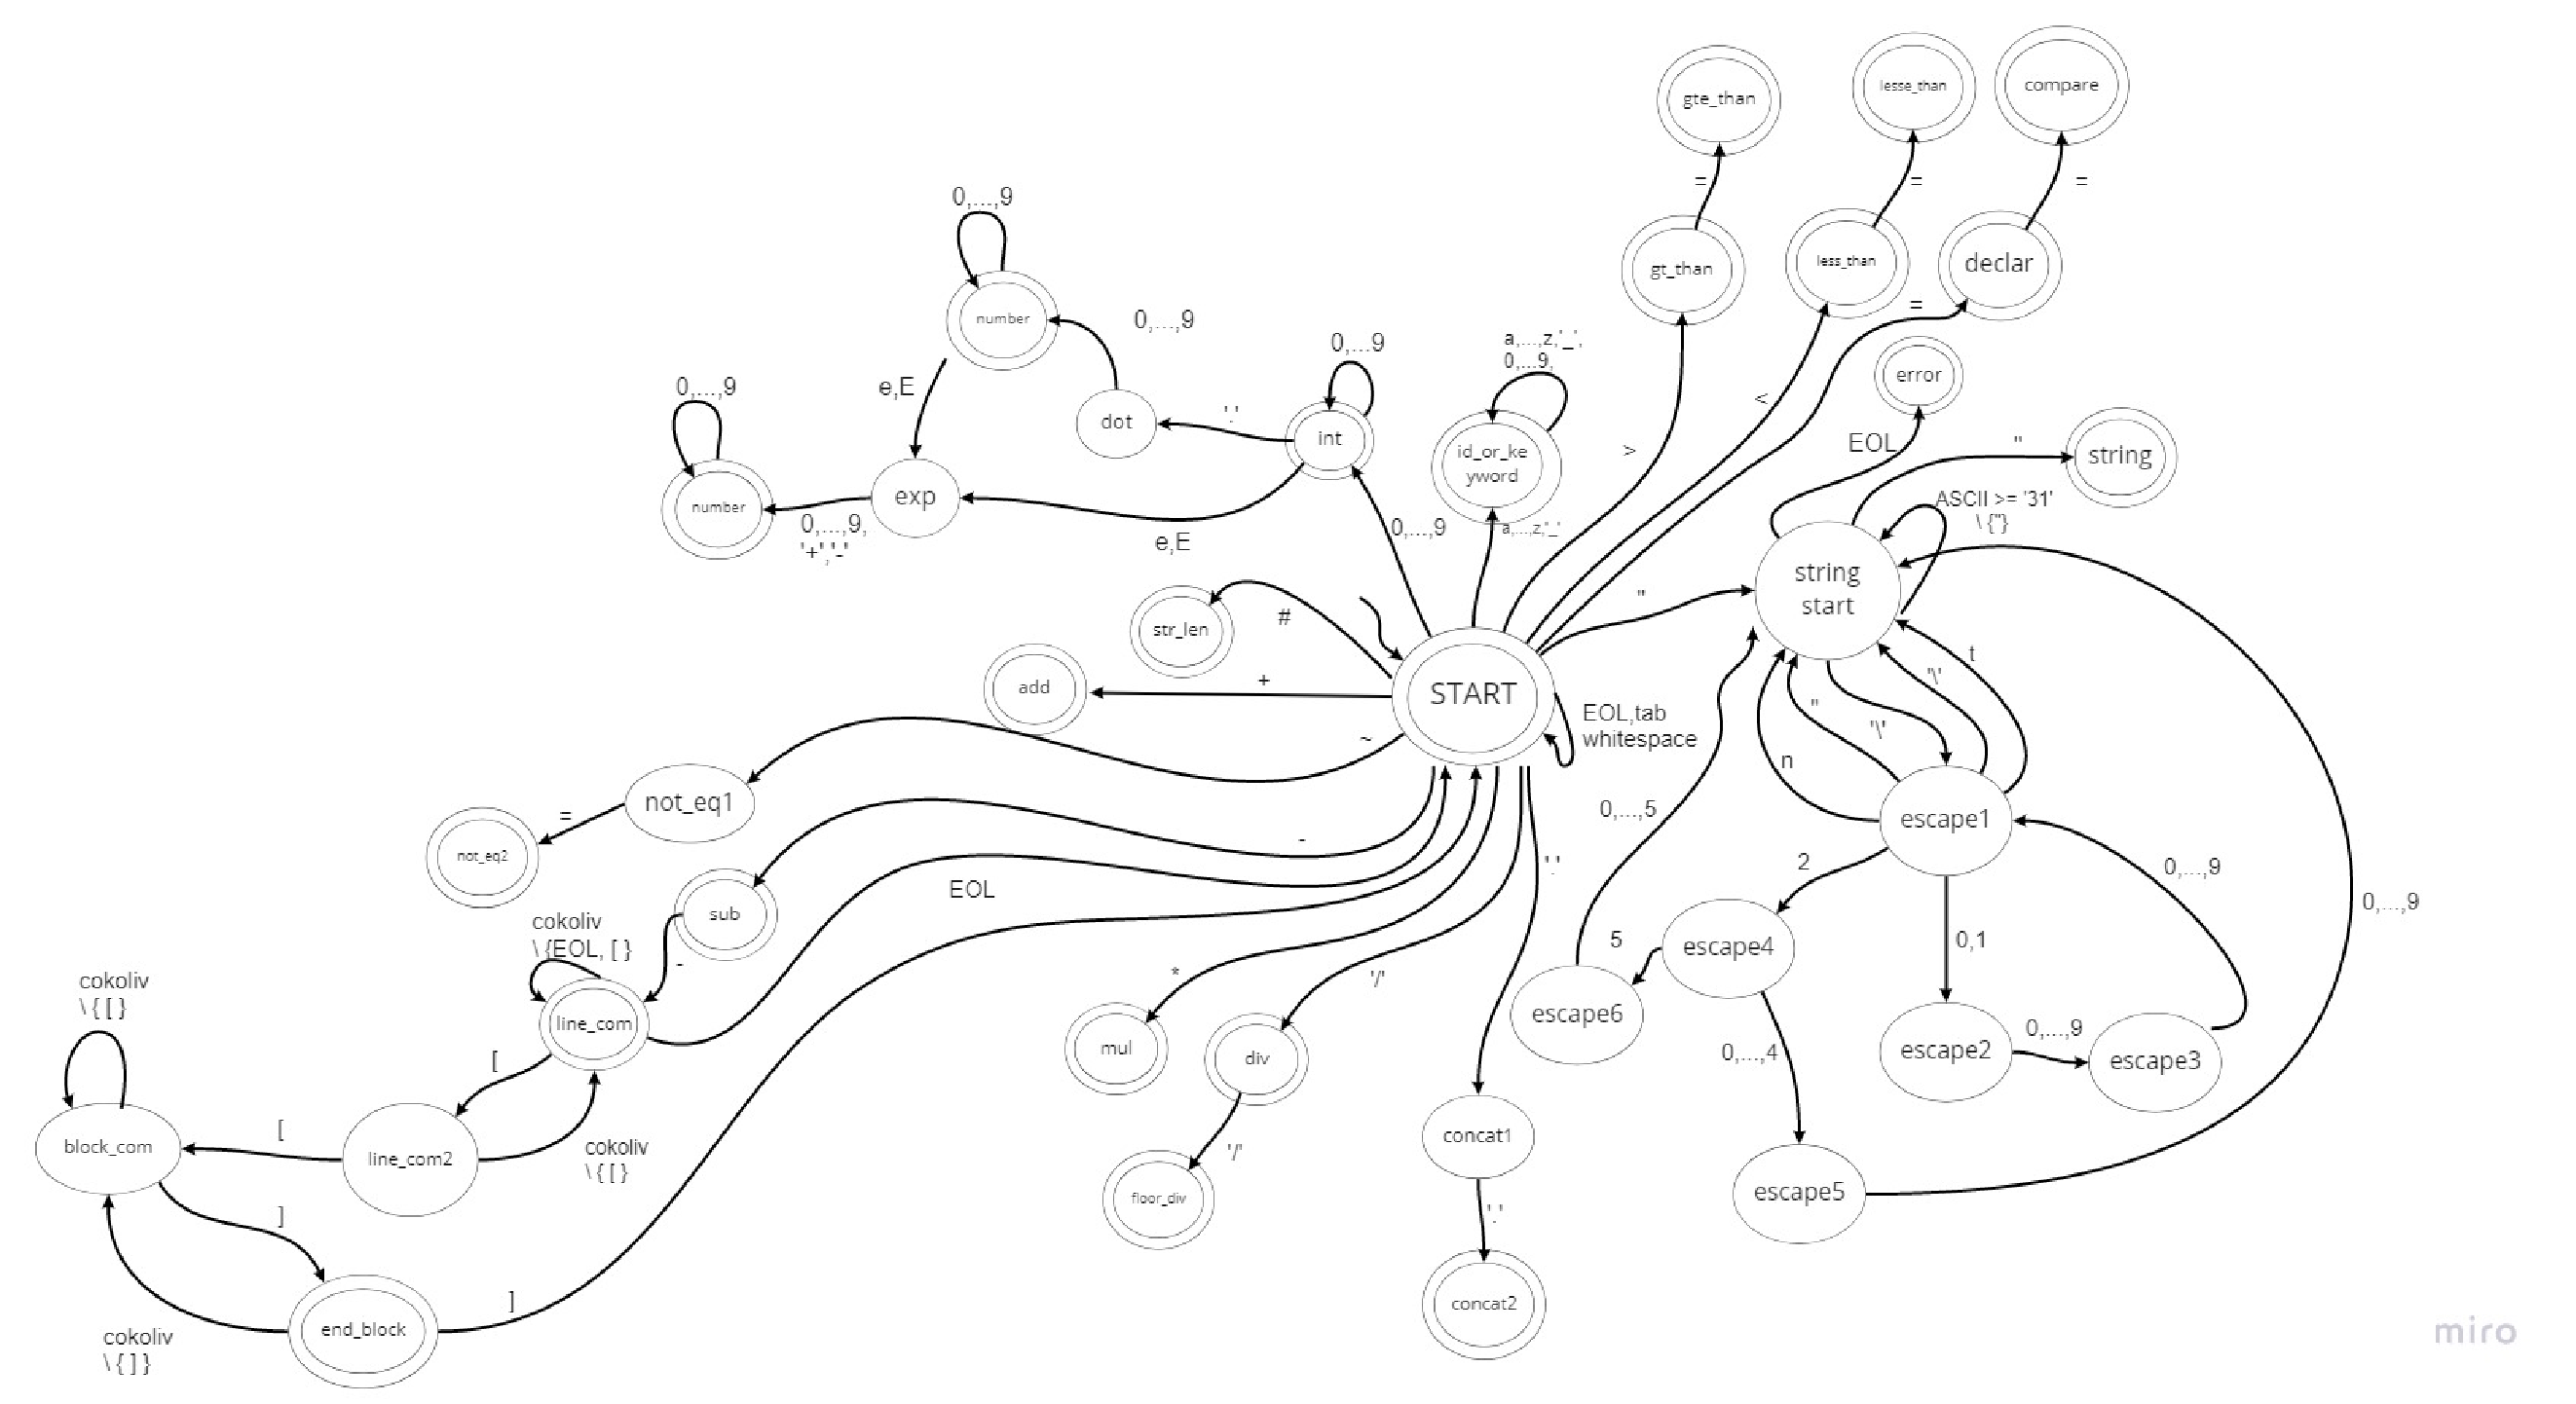
\includegraphics[width=\linewidth]{inc/automaton.pdf}

\subsection{Syntaktický analyzátor}

\subsubsection{LL-gramatika}

	\grule{PROG}{\ter{require} \ter{lit\_string} \nter{CODE}}
	\grule{CODE}{\ter{$\epsilon$}}
	\grule{CODE}{\nter{TOP\_ELEM} \nter{CODE}}
	\grule{TOP\_ELEM}{\nter{CALL}}
	\grule{TOP\_ELEM}{\nter{DECL}}
	\grule{TOP\_ELEM}{\nter{DEF}}
	\grule{DECL}{\ter{global} \ter{id} \ter{:} \ter{function} \ter{(}\nter{TYPE\_LIST}\ter{)} \nter{RET\_LIST}}
	\grule{DEF}{\ter{function} \ter{id} \ter{(} \nter{PARAM\_LIST} \ter{)} \nter{RET\_LIST} \nter{BODY} \ter{end}}
	\grule{CALL}{\ter{id} \ter{(} \nter{ARG\_LIST} \ter{)}} % TODO Toto by melo fungovat jenom pro konstanty jako parametry, volani funkci uvnitr funkci bude resit magic funkce
	\grule{RET\_LIST}{\ter{:} \nter{TYPE} \nter{NEXT\_TYPE}}
	\grule{RET\_LIST}{\ter{$\epsilon$}}
	\grule{TYPE\_LIST}{\nter{TYPE} \nter{NEXT\_TYPE}}
	\grule{TYPE\_LIST}{\ter{$\epsilon$}}
	\grule{NEXT\_TYPE}{\ter{,} \nter{TYPE} \nter{NEXT\_TYPE}}
	\grule{NEXT\_TYPE}{\ter{$\epsilon$}}
	\grule{TYPE}{\ter{nil}}
	\grule{TYPE}{\ter{integer}}
	\grule{TYPE}{\ter{number}}
	\grule{TYPE}{\ter{string}}
	\grule{ARG\_LIST}{\nter{ARG} \nter{NEXT\_ARG}}
	\grule{ARG\_LIST}{\ter{$\epsilon$}}
	\grule{NEXT\_ARG}{\ter{,} \nter{ARG} \nter{NEXT\_ARG}}
	\grule{NEXT\_ARG}{\ter{$\epsilon$}}
	\grule{ARG}{\ter{id}}
	\grule{ARG}{\ter{lit\_number}}
	\grule{ARG}{\ter{lit\_int}}
	\grule{ARG}{\ter{lit\_string}}
	\grule{ARG}{\ter{nil}}
	\grule{PARAM\_LIST}{\nter{PARAM} \nter{NEXT\_PARAM}}
	\grule{PARAM\_LIST}{\ter{$\epsilon$}}
	\grule{NEXT\_PARAM}{\ter{,} \nter{PARAM} \nter{NEXT\_PARAM}}
	\grule{NEXT\_PARAM}{\ter{$\epsilon$}}
	\grule{PARAM}{\ter{id} \ter{:} \nter{TYPE}}
	\grule{BODY}{\ter{$\epsilon$}}
	\grule{BODY}{\nter{STAT\_LIST}}
	\grule{STAT\_LIST}{\nter{VAR\_DECL} \nter{STAT\_LIST}}
	\grule{STAT\_LIST}{\nter{IF\_ELSE} \nter{STAT\_LIST}}
	\grule{STAT\_LIST}{\nter{WHILE} \nter{STAT\_LIST}}
	\grule{STAT\_LIST}{\ter{return} \nter{ARG\_LIST}}
	\grule{VAR\_DECL}{\ter{local} \ter{id} \ter{:} \nter{TYPE} \ter{=} \nter{INIT\_VAL}}
	\grule{IF\_ELSE}{\ter{if} \nter{EXPR} \ter{then} \nter{BODY} \ter{else} \nter{BODY} \ter{end}}
	\grule{WHILE}{\ter{while} \nter{EXPR} \ter{do} \nter{BODY} \ter{end}}

\subsubsection{LL-tabulka}

\begin{center}
	\scalebox{0.4}{
\begin{tabular}{| l || c | c | c | c | c | c | c | c | c | c | c | c | c | c | c | c | c | c | c | c | c | c | c | c | c |}
	                   & \ter{(} & \ter{)} & \ter{:} & \ter{,} & \ter{=} & \ter{do} & \ter{else} & \ter{end} & \ter{function} & \ter{global} & \ter{id} & \ter{if} & \ter{integer} & \ter{lit\_int} & \ter{lit\_number} & \ter{lit\_string} & \ter{local} & \ter{nil} & \ter{number} & \ter{require} & \ter{return} & \ter{string} & \ter{then} & \ter{while} & \ter{\$} \\\hline
	\nter{PROG}        &         &         &         &         &         &          &            &           &                &              &          &          &               &                &                   &                   &             &           &              & 1             &              &              &            &             & \\\hline
	\nter{CODE}        &         &         &         &         &         &          &            &           &    3           &         3    &  3       &          &               &                &                   &                   &             &           &              &               &              &              &            &             & 2\\\hline
	\nter{TOP\_ELEM}   &         &         &         &         &         &          &            &           &         6      &      5       &     4    &          &               &                &                   &                   &             &           &              &               &              &              &            &             & \\\hline
	\nter{DECL}        &         &         &         &         &         &          &            &           &                & 7            &          &          &               &                &                   &                   &             &           &              &               &              &              &            &             & \\\hline
	\nter{DEF}         &         &         &         &         &         &          &            &           & 8              &              &          &          &               &                &                   &                   &             &           &              &               &              &              &            &             & \\\hline
	\nter{CALL}        &         &         &         &         &         &          &            &           &                &              & 9        &          &               &                &                   &                   &             &           &              &               &              &              &            &             & \\\hline
	\nter{RET\_LIST}   &         &         &    10   &         &         &          &            &      11   &      11        &      11      &      11  &    11    &               &                &                   &                   &      11     &           &              &               &      11      &              &            &      11     & 11 \\\hline
	\nter{TYPE\_LIST}  &         &    11   &         &         &         &          &            &           &                &              &          &          &      12       &                &                   &                   &             &      12   & 12           &               &              &      12      &            &             & \\\hline
	\nter{NEXT\_TYPE}  &         &     15  &         &     14  &         &          &            &      15   &      15        &      15      &     15   &      15  &               &                &                   &                   &      15     &           &              &               &      15      &              &            &      15     & 15 \\\hline
	\nter{TYPE}        &         &         &         &         &         &          &            &           &                &              &          &          &      17       &                &                   &                   &             &      16   &      18      &               &              &     19       &            &             & \\\hline
	\nter{ARG\_LIST}   &         &    21   &         &         &         &          &      21    &      21   &                &              &      20  &          &               &      20        & 20                &  20               &             &      20   &              &               &              &              &            &             & \\\hline
	\nter{NEXT\_ARG}   &         &   23    &         &     22  &         &          &      23    &      23   &                &              &          &          &               &                &                   &                   &             &           &              &               &              &              &            &             & \\\hline
	\nter{ARG}         &         &         &         &         &         &          &            &           &                &              &     24   &          &               &         26     &      25           &           27      &             &      28   &              &               &              &              &            &             & \\\hline
	\nter{PARAM\_LIST} &         &    30   &         &         &         &          &            &           &                &              &      29  &          &               &                &                   &                   &             &           &              &               &              &              &            &             & \\\hline
	\nter{NEXT\_PARAM} &         &  32     &         &    31   &         &          &            &           &                &              &          &          &               &                &                   &                   &             &           &              &               &              &              &            &             & \\\hline
	\nter{PARAM}       &         &         &         &         &         &          &            &           &                &              &     33   &          &               &                &                   &                   &             &           &              &               &              &              &            &             & \\\hline
	\nter{BODY}        &         &         &         &         &         &          &    34      &     34    &                &              &          &    35    &               &                &                   &                   &      35     &           &              &               &    35        &              &            &      35     & \\\hline
	\nter{STAT\_LIST}  &         &         &         &         &         &          &            &           &                &              &          &    37    &               &                &                   &                   &      36     &           &              &               &      39      &              &            &      38     & \\\hline
	\nter{VAR\_DECL}   &         &         &         &         &         &          &            &           &                &              &          &          &               &                &                   &                   &      40     &           &              &               &              &              &            &             & \\\hline
	\nter{IF\_ELSE}    &         &         &         &         &         &          &            &           &                &              &          &   41     &               &                &                   &                   &             &           &              &               &              &              &            &             & \\\hline
	\nter{WHILE}       &         &         &         &         &         &          &            &           &                &              &          &          &               &                &                   &                   &             &           &              &               &              &              &            &    42       & \\

\end{tabular}
}
\end{center}

\subsubsection{Případy nepokryté LL-gramatikou} %TODO



\subsection{Sémantické kontroly}%TODO

\subsection{Generování kódu}%TODO

\subsection{Tabulka symbolů}%TODO

\end{document}
